%% main.tex — MSE Project Report: HiUni
%% Dokumentklasse msereport (1:1-Nachbau der Word-Vorlage template.docx).
%% Uebersetzen mit:  latexmk -pdf main.tex     (oder -lualatex fuer echtes Arial)
\documentclass{msereport}

% --- Architekturdiagramm (Abschnitt 3) --------------------------------------
\usepackage{tikz}
\usetikzlibrary{arrows.meta,calc,positioning}

% Umbruchstelle in langen Bezeichnern (ohne Trennstrich)
\newcommand{\bk}{\allowbreak}

% Rahmen-/Fuellfarben der Diagrammschichten
\definecolor{diaui}{HTML}{4F46E5}     % UI
\definecolor{diavm}{HTML}{7C3AED}     % Presentation
\definecolor{diarepo}{HTML}{0F766E}   % Domain/Daten
\definecolor{diadata}{HTML}{B45309}   % Persistenz & Netzwerk
\definecolor{diaext}{HTML}{6B7280}    % externe Systeme
\definecolor{diafcm}{HTML}{B31B1B}    % eigener Push-Server

\tikzset{
  dbox/.style={draw=#1, line width=0.3pt, fill=#1!10, rounded corners=2pt,
               anchor=north west, align=left, inner xsep=3pt, inner ysep=3pt,
               text=msetext, font=\fontsize{6.4pt}{7.4pt}\selectfont},
  dui/.style={dbox=diaui},
  dvm/.style={dbox=diavm},
  drepo/.style={dbox=diarepo},
  ddata/.style={dbox=diadata},
  dext/.style={dbox=diaext, font=\fontsize{6pt}{6.9pt}\selectfont},
  dfcm/.style={dbox=diafcm, dashed, font=\fontsize{6.2pt}{7.2pt}\selectfont},
  arr/.style={draw=msetext, line width=0.3pt,
              -{Stealth[length=3.4pt,width=2.4pt]}},
  lbl/.style={font=\fontsize{5.7pt}{6.6pt}\selectfont, text=msetext,
              fill=white, inner sep=1pt, align=left},
  lblr/.style={lbl, align=right},
  lay/.style={rotate=90, anchor=center, text=#1,
              font=\bfseries\fontsize{6pt}{6.9pt}\selectfont},
}

% Umbruch an bestehenden Bindestrichen erlauben (wie in Word); die
% Silbentrennung selbst bleibt aus, damit keine falschen deutschen
% Trennstellen entstehen.
\AtBeginDocument{\exhyphenpenalty=50\relax}

\hypersetup{
  pdftitle={HiUni — MSE Project Report},
  pdfauthor={Kjell Karstens, Johann Brosthaus},
}

\begin{document}

% ===========================================================================
%  Titelblock
% ===========================================================================
\msetitleblock{Project Report}{HiUni — Campus-App für die Universität Hildesheim}

{\mseleadfont Team:}
\par\vspace{10pt}

\begin{msetblr}[l]{
  colspec={Q[l,wd=5.6304cm] Q[l,wd=10.0330cm]},
  row{1}={bg=msetablered},
}
  Name & Student ID \\
  Kjell Karstens & \msestrut \\
  Johann Brosthaus & \msestrut \\
\end{msetblr}

% ===========================================================================
\section{Use Case}
% ===========================================================================

\begin{itemize}
  \item \textbf{Problemstellung:} Studierende der Universität Hildesheim
        benutzen täglich ein Dutzend digitale Dienste: Mensaplan,
        LSF-Notenübersicht, Learnweb-Abgaben, Bibliotheks-Raumbuchung,
        Hochschulsport, Unikino, Uni-Mail, Stundenplan. Alle liegen auf
        getrennten Webseiten, ohne zentrale Übersicht und ohne universelles
        Login. Wer mehrfach täglich nach Essen, Abgaben oder Mails schaut, meldet
        sich für jeden Dienst neu an, und das auf dem Smartphone, für das die
        meisten dieser Seiten nicht gemacht sind.
  \item \textbf{Motivation:} Wir wollten die Dienste, die wir selbst mehrmals
        täglich brauchen, an einem Ort haben, und so, dass auch andere
        Studierende sie benutzen können. Vergleichbare Apps existieren
        (z.\,B.\ Studo), decken die Uni Hildesheim aber nicht in der Tiefe ab,
        die den Alltag wirklich vereinfacht: keine LSF-Noten, keine
        Gruppenraum-Buchung, kein Uni-Mail-Postfach. Und das Projekt war die
        Gelegenheit, die MSE-Inhalte (Android-Architektur, Compose, Lifecycle,
        Persistenz, Testing) an einem Problem auszuprobieren, das uns selbst
        betrifft.
  \item \textbf{Real-World-Relevanz:} Das Zielbild aus unserer
        Projektbeschreibung lautet: ,,Eine Studentin der Uni Hildesheim soll in
        unter 10 Sekunden nach App-Start wissen, was sie heute zu tun hat, was
        es in der Mensa gibt, welche Mails ungelesen sind und welche Abgaben
        anstehen, ohne sich irgendwo neu anmelden zu müssen.`` Heute braucht
        man dafür fünf Webseiten und vier Logins.
  \item \textbf{Bewusste Abgrenzung:} HiUni ist \emph{kein} Ersatz für LSF und
        Learnweb: die App aggregiert öffentliche Inhalte und Login-Sessions; wo
        eine echte Verwaltungsaktion nötig ist (Sportkurs-Anmeldung), verweist
        sie auf die offizielle Seite. Sie ist auch keine Bewertungsplattform und
        keine Anwendung der Uni-IT, sondern ein privates Studierendenprojekt im
        MSE-Modul, nicht mit der Uni-IT abgestimmt. Cross-Platform wurde bewusst
        nicht gewählt: native Android war Kursvorgabe und Lernziel.
\end{itemize}

\msegap

% ===========================================================================
\section{UX Design and Target Group}
% ===========================================================================

\subsection{Target Group}

\begin{itemize}
  \item \textbf{Primärnutzer:} Studierende der Universität Hildesheim, alle
        Semester und Studiengänge. Absichtlich breit geschnitten, weil Mensa,
        Mail, Stundenplan und Bibliothek studiengangsunabhängig sind.
  \item \textbf{Sekundärnutzer:} Mitarbeitende mit Lehrauftrag, die in der Mensa
        essen oder ihr Uni-Postfach prüfen; benutzbar, aber nicht der
        Designfokus, denn Prüfungs-, Noten- und Abgabe-Features sind auf
        Studierende zugeschnitten.
  \item \textbf{Ausdrücklich nicht Zielgruppe:} Studierende anderer Hochschulen
        (alle Endpunkte, Scraper und Zugangsdaten sind Uni-Hildesheim-spezifisch)
        und iOS-Nutzer.
  \item \textbf{User Needs (in Klammern der heutige Workaround):} Wissen, was
        heute anliegt (LSF-Stundenplan im Browser, kein Tagesüberblick);
        Mensaplan sehen (separate STW-ON-Webseite); ungelesene Mails prüfen
        (eigenes Webmail-Login mit RZ-Kennung); Abgaben im Blick behalten
        (Learnweb, CAS-Login pro Besuch); Noten und Schnitt überblicken
        (LSF-Notenspiegel, im Kopf aggregieren); freien Gruppenraum finden und
        buchen (ubwww mit eigenem Session-Handling); Sportkurs finden
        (HSP-Programmseite, Buchung hinter eigenem Login).
  \item \textbf{Usage-Szenario (eigene Ausformulierung des Zielbilds aus
        Abschnitt 1):} Eine Studentin öffnet HiUni morgens im Bus. Sie sieht auf
        dem Home-Screen die nächste Vorlesung mit Countdown und Raum, darunter
        das heutige Mensa-Angebot, die ungelesenen Mails und die nächste fällige
        Abgabe. Sie tippt auf die Abgabe, sieht die Frist, und legt sich
        unterwegs noch einen Gruppenraum für den Nachmittag auf ihren Namen,
        ohne sich in vier Portalen anzumelden.
\end{itemize}

\subsection{Mockups}

\begin{itemize}
  \item Als Design-Referenz diente ein High-Fidelity-HTML/CSS-Mock
        (\emph{Uni Hi.html}) mit 17 Screens, mit \emph{Claude Design} erzeugt und
        von Hand nachgeschärft; die KI-Reflexion dazu steht in Abschnitt 4.2. Aus
        ihm wurden Farbsystem (OKLCH-Werte als sRGB-Konstanten),
        Typografie-Skala, Corner-Radii und das Home-Layout ins Compose-Theme
        übersetzt.
  \item Die drei Kern-Workflows der folgenden Tabelle stammen daher; die Bilder
        sind direkt aus dem Mock gerendert.
\end{itemize}

\msegap

\begin{msetblr}[l]{
  colspec={Q[l,wd=3.4572cm] Q[l,wd=6.2794cm] Q[l,wd=5.5033cm]},
  row{1}={bg=msered2},
  cells={font=\msesmallfont},
}
  Screen & Mockup & Addresses which user need? \\
  Home (Tagesüberblick) & 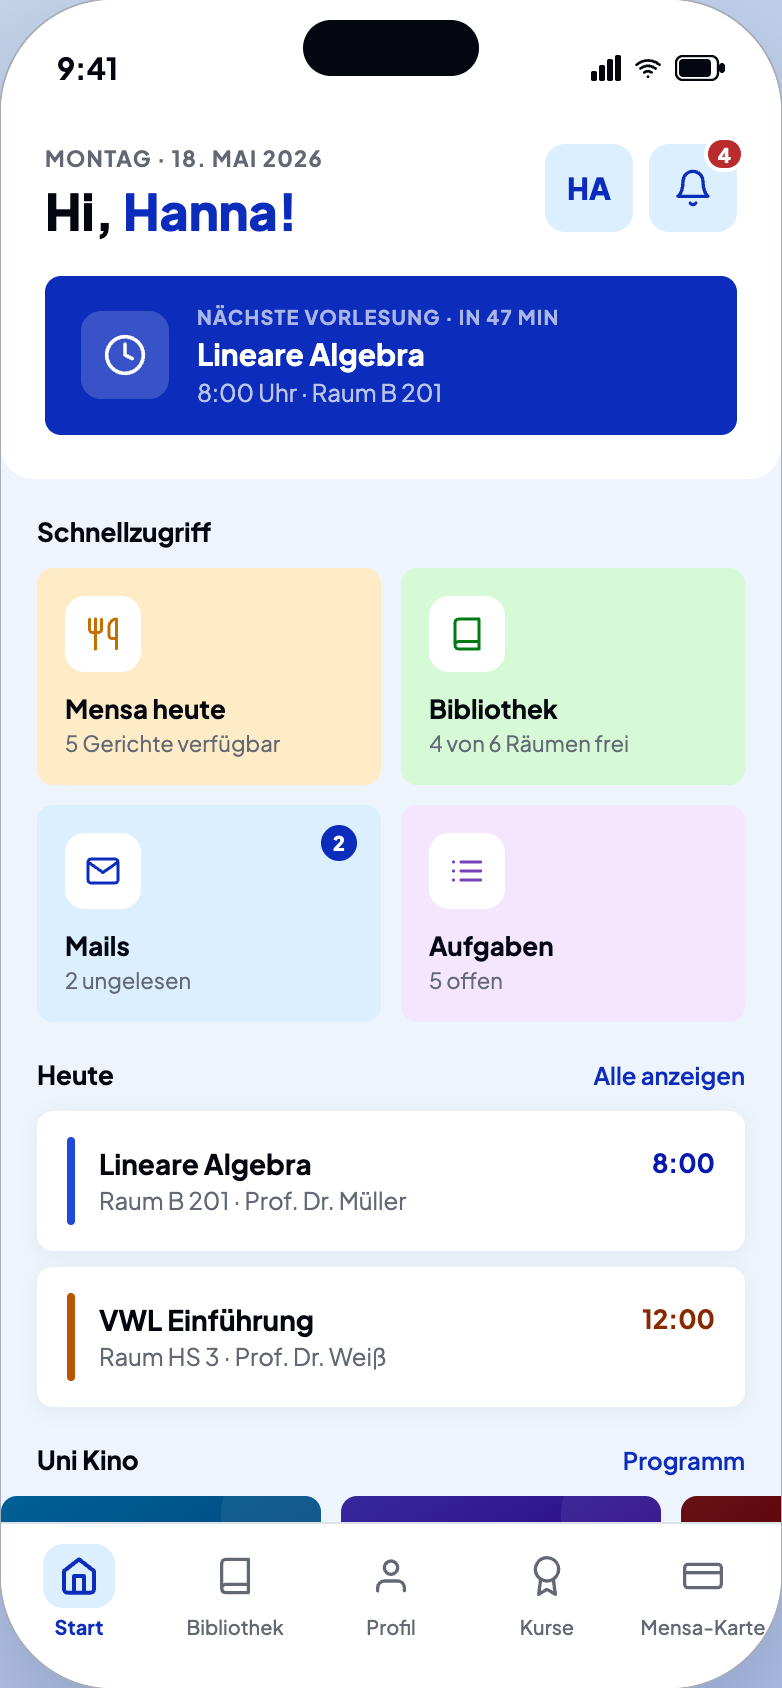
\includegraphics[width=2.35cm]{assets/mock-home.png} & Tagesüberblick ohne Mehrfach-Login in einem Screen: was steht an, was gibt es zu essen, was ist offen \\
  Bibliothek / Gruppenraum & 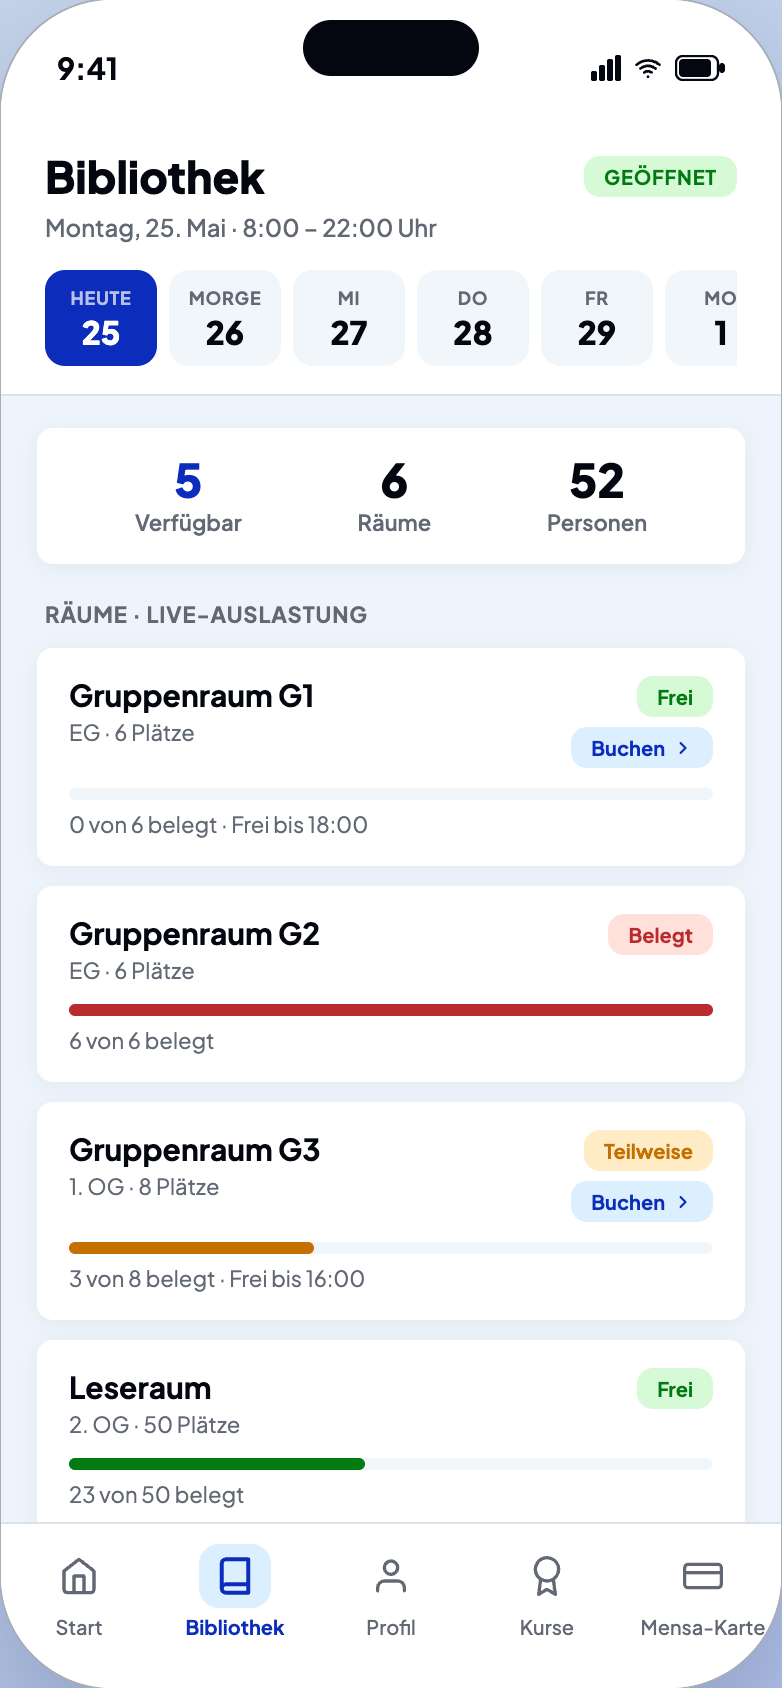
\includegraphics[width=2.35cm]{assets/mock-bib.png} & Freien Lernraum finden und direkt buchen, statt die ubwww-Seite auf dem Handy zu bedienen \\
  Aufgaben und Noten & 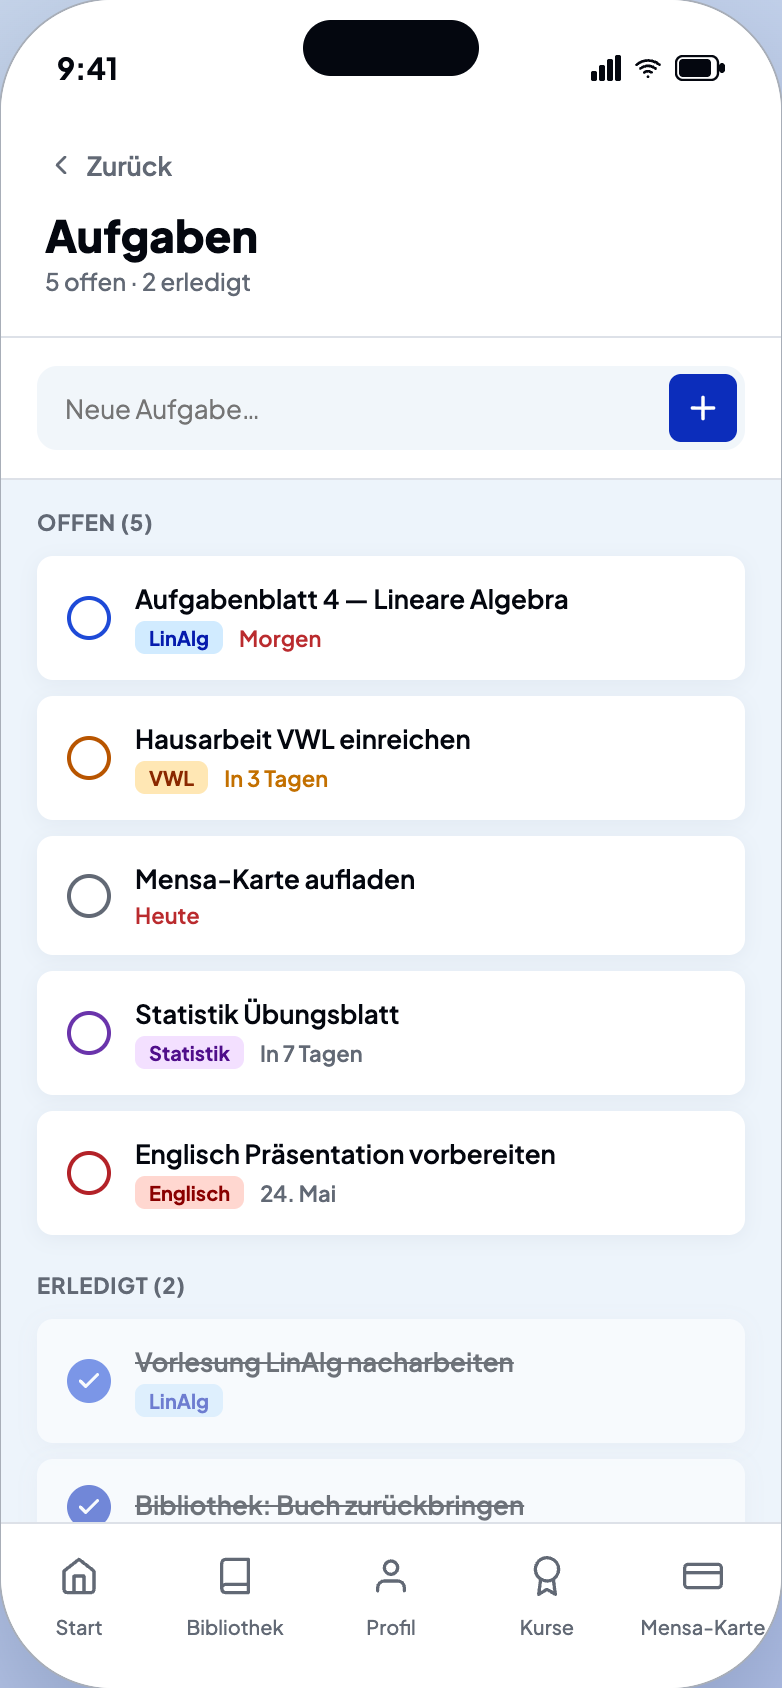
\includegraphics[width=2.35cm]{assets/mock-todo.png}\hspace{4pt}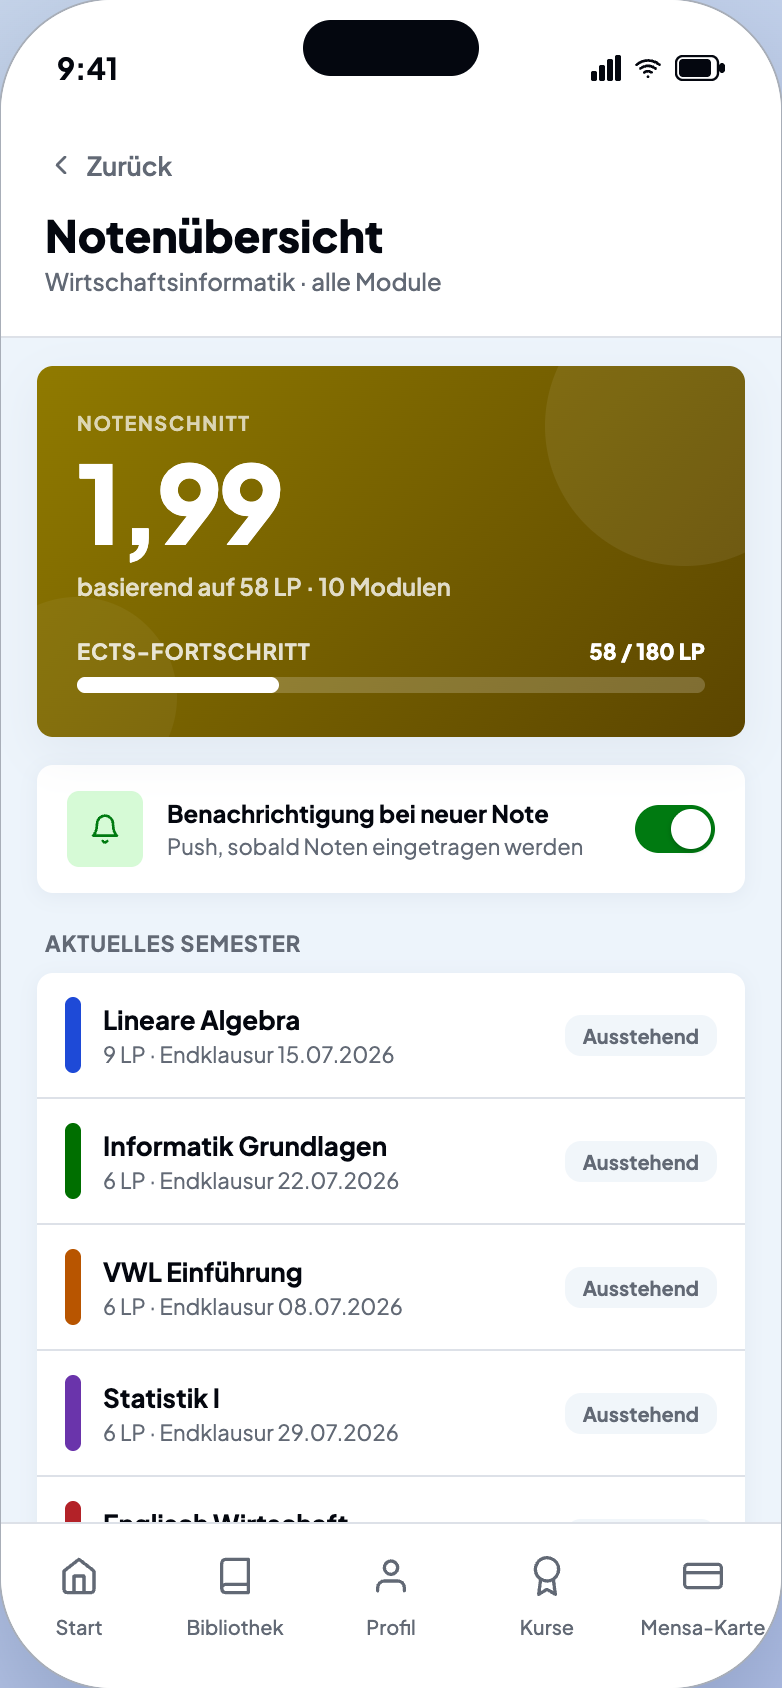
\includegraphics[width=2.35cm]{assets/mock-noten.png} & Abgaben und Noten im Blick, ohne pro Besuch neu über CAS einzuloggen \\
\end{msetblr}

\msevspace{10pt}\mseblank

\subsection{Design Rationale}

\begin{itemize}
  \item \textbf{Bewusst weggelassen bzw.\ vereinfacht:} Der Mock hatte 17
        Screens; gestartet sind wir mit acht Navigationszielen (Home, Kalender,
        Mensa, Kino, Bib, Mail, Einstellungen, Über). Klausuren, Noten, Sport und
        das Push-Center kamen später nach, Lerngruppen und Campus-Plan sind nicht
        gebaut: die Restaufwände passten nicht ins Zeitbudget, und Lerngruppen
        ohne Backend wären eine lokale Notizliste geblieben. Das
        In-App-Tweaks-Panel (Akzentfarbe, Begrüßungstext) haben wir verworfen,
        weil es die Einstellungen doppelt hätte. Der Über-Screen ist bewusst ein
        Minimalstub geblieben.
  \item \textbf{Design-System statt Standardkomponenten:} Pillen, Badges und den
        ,,Pillow``-Indikator der Bottom-Navigation haben wir aus
        \texttt{Surface} und \texttt{Text} von Hand nachgebaut, statt
        Material-3-Komponenten mit abweichender Anmutung zu nehmen. Kostet mehr
        Code, hält aber Abstände, Radien und Farbrollen über alle Screens
        konsistent.
  \item \textbf{UX-Entscheidung gegen den KI-Vorschlag:} Für die Tagesansicht des
        Kalenders generierte die KI ein vollständiges Stundenraster von 8 bis 22
        Uhr mit Positionsberechnung pro Termin. Im Pair-Review haben wir das für
        die damalige Projektphase als over-engineered zurückgewiesen und auf eine
        Agenda-Liste reduziert; der Rest der Feature-Welle war wichtiger als eine
        schöne Tagesansicht. In einer späteren Polish-Phase kam dann doch ein
        farbkodiertes Stundenraster (8--18 Uhr). Der Vorschlag kam also nur zu
        früh, und im Review prüfen wir seitdem auch, ob etwas in die aktuelle
        Projektphase passt.
\end{itemize}

\msegap

% ===========================================================================
\section{System Architecture Diagram}
% ===========================================================================

% Diagramm gemeinsam mit KI entworfen, von Hand nachgeführt — Anpassungen:
% Boxen/Pfeile hier direkt editierbar.
% Geometrie: alle Knoten mit anchor=north west an festen (x,y)-Positionen in cm,
% Schichten bei y = 0 / -2.70 / -5.30 / -7.85 / -11.70.
{\hbadness=10000 \hfuzz=30pt
\begin{tikzpicture}[x=1cm, y=1cm]

  \tikzset{
    bignode/.style={font=\fontsize{7.4pt}{8.8pt}\selectfont},
    biarr/.style={arr, {Stealth[length=3.4pt,width=2.4pt]}-{Stealth[length=3.4pt,width=2.4pt]}},
  }

  % ---------- Schicht-Beschriftungen (links) --------------------------------
  \node[lay=diaui]   at (0.30,-0.55) {UI};
  \node[lay=diavm]   at (0.30,-2.55) {Presentation};
  \node[lay=diarepo] at (0.30,-4.55) {Domain};
  \node[lay=diadata] at (0.30,-6.75) {Daten \& Infra};
  \node[lay=diaext]  at (0.30,-9.65) {Extern};

  % ---------- Schicht 1: UI -------------------------------------------------
  \node[dui, bignode, text width=13.6cm, minimum height=1.05cm] (UI) at (0.9,0)
    {{\bfseries Compose-UI (Single Activity) + Glance-Home-Widgets}\\
     rendern \texttt{UiState}, senden User-Aktionen; Widgets lesen Repository-Flows direkt};

  % ---------- Schicht 2: ViewModels ----------------------------------------
  \node[dvm, bignode, text width=13.6cm, minimum height=1.05cm] (VM) at (0.9,-2.0)
    {{\bfseries Feature-ViewModels (\texttt{@HiltViewModel}), inkl.\ HomeViewModel}\\
     halten je Screen einen \texttt{UiState} als StateFlow, rufen Repository-Funktionen};

  % ---------- Schicht 3: Repositories --------------------------------------
  \node[drepo, bignode, text width=13.6cm, minimum height=1.05cm] (REPO) at (0.9,-4.0)
    {{\bfseries Feature-Repositories als Single Source of Truth}\\
     TTL-Refresh, Mapping HTML/JSON auf Room-Entities, liefern Flows nach oben};

  % ---------- Schicht 4: Daten \& Infrastruktur -----------------------------
  \node[ddata, bignode, text width=6.5cm, minimum height=1.35cm] (STORE) at (0.9,-6.0)
    {{\bfseries Room + SQLCipher, DataStore}\\
     verschlüsselte DB (Schema 35, 34 Migrationen),\\
     Einstellungen und Zugangsdaten};

  \node[ddata, bignode, text width=6.5cm, minimum height=1.35cm] (NET) at (8.0,-6.0)
    {{\bfseries Netzwerk, WorkManager, CasSession}\\
     OkHttp + Jsoup-Scraper, Hintergrund-Worker,\\
     CAS-SSO mit Silent-Renewal};

  % ---------- Schicht 5: externe Systeme -----------------------------------
  \node[dext, bignode, text width=9.6cm, minimum height=1.15cm] (EXT) at (0.9,-9.0)
    {{\bfseries Uni-Systeme (kein API, per Scraping / Protokoll)}\\
     LSF + CAS, Learnweb, STW-Mensa, ubwww-Bib, Uni-Mail (IMAP/SMTP)};

  \node[dfcm, bignode, text width=3.5cm, minimum height=1.15cm] (FCM) at (11.0,-9.0)
    {{\bfseries FCM-Tickle-Server}\\
     (FastAPI; Deployment\\ ausstehend)};

  % ---------- Pfeile --------------------------------------------------------
  \draw[biarr] (7.0,-1.05) -- (7.0,-2.0);
  \node[lbl, anchor=west] at (7.15,-1.52) {$\downarrow$ Aktionen \quad $\uparrow$ UiState (StateFlow)};

  \draw[biarr] (7.0,-3.05) -- (7.0,-4.0);
  \node[lbl, anchor=west] at (7.15,-3.52) {$\downarrow$ \texttt{refresh()} \quad $\uparrow$ \texttt{Flow<Entity>}};

  \draw[biarr] (3.5,-5.05) -- (3.5,-6.0);
  \node[lbl, anchor=west] at (3.65,-5.52) {Query / \texttt{upsert}};

  \draw[arr] (11.2,-5.05) -- (11.2,-6.0);
  \node[lbl, anchor=west] at (11.35,-5.52) {Sync anstoßen};

  \draw[arr] (9.3,-7.35) -- (9.3,-9.0);
  \node[lblr, anchor=east] at (9.15,-8.1) {HTTPS, CAS-Cookie,\\Scraping (rate-limited)};

  \draw[arr, dashed] (12.7,-9.0) -- (12.7,-7.35);
  \node[lbl, anchor=west] at (12.85,-8.1) {stiller Tickle\\(geplant)};

\end{tikzpicture}
\par}
\vspace{4pt}
{\msesmallfont\itshape Lesart: Pfeile nach unten sind Aufrufe, Pfeile nach oben
sind Datenströme (Flows).\par}

\subsection{Architecture Justification}

\begin{itemize}
  \item \textbf{Warum diese Struktur?} Die App ist strikt geschichtet (Compose
        $\to$ ViewModel $\to$ Repository $\to$ Room/Netzwerk), aber
        \emph{feature-first} paketiert: jedes der 21 Feature-Packages bündelt
        Entities, DAOs, Repositories, ViewModels und Screens an einem Ort. Das
        Repository ist die einzige Quelle der Wahrheit; die UI liest nie vom
        Netz, sondern aus Room-Flows, weshalb jeder Screen sofort Inhalt hat und
        die App offline benutzbar bleibt. Cross-Feature-Zugriffe sind per
        Konvention verboten, mit zwei dokumentierten Ausnahmen:
        \texttt{feature.home} (kombiniert elf Repositories) und
        \texttt{feature.widgets} (Glance kennt keine ViewModels). Weil fünf
        Fremdsysteme per HTML-Scraping angebunden sind (LSF, Learnweb, ubwww,
        unifilm, Hochschulsport), liegen HTTP-Client, Höflichkeits-Drossel,
        CAS-Session und Hintergrund-Worker außerhalb der Features; sonst hätte
        jeder Scraper eigene Rate-Limit- und Session-Logik. Der FCM-Tickle-Server
        ist absichtlich ein separater, inhaltsleerer Kasten: er kennt nur
        Device-Tokens und schickt einen reinen ,,schau nach``-Impuls, sodass nie
        Zugangsdaten oder Mailinhalte einen fremden Server berühren. Er ist
        implementiert und getestet, aber nicht produktiv deployed; bis dahin
        läuft der Mail-Sync über die periodischen WorkManager-Worker.
        Sicherheitskritische Daten liegen in einer SQLCipher-verschlüsselten
        Room-Datenbank mit Schlüssel aus dem Android-Keystore.
  \item \textbf{Verworfene Alternativen:} (1) \emph{Layer-first mit mehreren
        Gradle-Modulen}: Single-Module baut bei unserer Größe schneller und die
        Feature-Verantwortung zerfasert nicht; der Preis ist fehlende
        Compile-Time-Isolation, die Packages sind aber 1:1 überführbar.
        (2) \emph{Retrofit + Moshi}: lohnt neben überwiegend HTML-Scraping für
        eine Handvoll JSON-Endpunkte nicht, OkHttp plus kotlinx.serialization
        genügen. (3) \emph{Koin statt Hilt}: spart Boilerplate, kostet aber die
        Compile-Time-Prüfung des Abhängigkeitsgraphen. (4) \emph{Eine gemeinsame
        Kalendertabelle}: der Diskriminator-Ansatz bricht die
        Feature-Trennung, gepinnte Einträge sind jetzt Snapshots in einer eigenen
        Tabelle. (5) \emph{AGP 9}: Hilt brach damit komplett, zurück auf
        AGP 8.7 + Kotlin 2.0 + KSP1.
  \item \textbf{Walk-Through (Szenario aus 2.1: ,,App morgens öffnen``):}
        (1) Der Tickle-Server soll alle 15 Minuten eine stille
        High-Priority-FCM-Data-Message ohne Nutzdaten schicken (Server gebaut,
        Deployment steht aus; aktuell startet stattdessen der periodische Worker).
        (2) Der \texttt{HiUniMessagingService} empfängt sie, holt seine
        Abhängigkeiten über einen Hilt-\texttt{EntryPoint} (Firebase instanziiert
        ihn selbst), prüft Vorbedingungen und reiht einen \emph{expedited}
        \texttt{MailPushSyncWorker} ein; nicht der Service arbeitet, weil dessen
        Prozess sofort enden kann. (3) Der Worker ruft
        \texttt{EmailRepository.refresh()} und klassifiziert Netzwerkfehler als
        \texttt{retry}, Auth-Fehler als \texttt{failure}; parallel besorgt sich
        der \texttt{LsfSyncWorker} über \texttt{CasSession} ein Service-Ticket
        mit Silent-Renewal. (4) Alle HTTP-Aufrufe gehen durch den gemeinsamen
        OkHttp-Client mit Cookie-Jar und \texttt{PolitenessInterceptor}; HTML
        parst Jsoup, die Mensa-Antwort kotlinx.serialization. (5) Ergebnisse
        werden in Room upserted, ein Schreibvorgang, an dem alle Beobachter
        hängen; die DAOs emittieren neue Flows, die Repositories reichen sie
        weiter. (6) Das \texttt{HomeViewModel} kombiniert die Flows aus elf
        Feature-Repositories (Kalender, Mensa, Mail, Aufgaben, \dots) zu einem
        \texttt{HomeUiState}. (7) Der \texttt{HomeScreen} collected ihn
        \texttt{withLifecycle} und zeichnet Banner, Mensa-Karte und Mail-Badge;
        das Stundenplan-Widget liest denselben Flow über den Widget-EntryPoint.
\end{itemize}

\subsection{Third-Party Libraries}

In einem Satz: Hilt verdrahtet die App, Room und SQLCipher speichern
verschlüsselt, OkHttp und Jsoup holen und parsen die Uni-Seiten, Jakarta Mail
spricht IMAP/SMTP, kotlinx.serialization und biweekly lesen JSON und iCal, Coil
lädt Bilder, Firebase liefert den Push-Transport, und MockK/Turbine/Robolectric
tragen die Tests. Alles darunter löst genau eine Aufgabe, die man sonst selbst
bauen müsste.
\par\vspace{6pt}

{\itshape Neben den Plattform-Bausteinen von Google/AndroidX (Compose,
Navigation, Lifecycle, DataStore, WorkManager, Glance, Biometric, Window/WindowSizeClass,
Fragment für BiometricPrompt, SplashScreen, Palette für Poster-Farben, Material-Icons,
Google-Fonts) und den Kotlin-Coroutines, die wir als Teil der Architekturentscheidung
und nicht als Fremdbibliotheken zählen, sind folgende Dritt-Bibliotheken im Einsatz.
Zusätzlich, aber ohne Einfluss auf die Fachlichkeit: Timber (Logging) und LeakCanary
(nur im Debug-Build).\par}
\vspace{6pt}

\begin{msetblr}[l]{
  colspec={Q[l,wd=3.8100cm] Q[l,wd=5.7150cm] Q[l,wd=5.7150cm]},
  row{1}={bg=msered2},
  cells={font=\msesmallfont},
}
  Library & Purpose & Why this one (over alternatives)? \\
  Hilt / Dagger 2.56 & DI, \texttt{@HiltViewModel}, \texttt{@HiltWorker}, EntryPoints für Widgets und Push-Service & Compile-Time-Prüfung des Abhängigkeitsgraphen statt Laufzeit-Überraschungen \\
  Room 2.6.1 (+ KSP) & SQLite-Zugriff, eine AppDatabase, Entities und DAOs im Feature, versionierte Migrationen & Typsichere Queries und Flow-Integration; KSP1, weil Room 2.6.1 mit KSP2 nicht kompiliert \\
  SQLCipher (sqlcipher-android 4.6.1) & Verschlüsselung der gesamten Room-Datenbank & Mail-Cache, Noten und Prüfungsdaten liegen auf Platte; Prefs allein lassen die DB offen \\
  OkHttp 4.12 (+ Logging-Interceptor) & HTTP-Client für Scraper und APIs, Cookie-Jar, Cache, Höflichkeits-Interceptor & Cookies, Pool und Cache eingebaut; mit \texttt{HttpURLConnection} wäre das Handarbeit \\
  Jsoup 1.18.1 & HTML-Parsing für LSF, Learnweb, ubwww, unifilm, Hochschulsport & Robuste CSS-Selektoren auf kaputtem Uni-HTML statt Regex \\
  Angus Mail 2.0.3 / Jakarta Mail API 2.1.3 & IMAP- und SMTP-Client des Mail-Features & Protokollkorrekt inklusive IDLE und SPECIAL-USE; eigener Parser wäre Wochen Arbeit \\
  kotlinx.serialization 1.7.3 & Typsichere DTOs für JSON-Endpunkte (Mensa, TMDB) & Kotlin-nativ, kein Reflection-Overhead; Retrofit/Moshi lohnen erst bei mehr Endpunkten \\
  Coil 2.7.0 (coil-compose) & Asynchrones Laden der Kino-Poster & Cache, Nebenläufigkeit und Compose-Integration fertig \\
  Firebase Cloud Messaging (firebase-bom 33.7.0) & Empfang der stillen Tickle-Data-Messages unseres Push-Servers & Einziger Weg aus dem Doze ohne Polling; genutzt wird nur der Transport, keine Analytics \\
  biweekly 0.6.8 & iCalendar-Parsing (RFC 5545) des Learnweb-Feeds als Zweitquelle für Fristen & Korrekte RRULE- und EXDATE-Expansion ist ein eigenes Projekt \\
  MockK 1.13.13, Turbine 1.1.0, Robolectric 4.13 & Unit-Tests: Kotlin-Mocking, Flow-Assertions, Android-Tests auf der JVM & MockK versteht Kotlin-Idiome, Turbine macht StateFlow-Tests lesbar, Robolectric spart den Emulator \\
\end{msetblr}

\msegap

\subsection{Der Tickle-Server: Idee und Stand}

Neue Uni-Mails schnell zu bemerken, kollidiert mit Android: Aus dem
Doze-Modus darf eine App nicht im Minutentakt selbst nachschauen. Der übliche
Ausweg wäre ein Server, der die Postfächer überwacht und bei neuer Mail eine
Push-Nachricht mit Inhalt schickt, aber dann lägen Zugangsdaten und
Mailinhalte auf fremder Infrastruktur. Unser \emph{Tickle}-Server umgeht genau
das: Er kennt ausschließlich FCM-Device-Tokens, also nur ,,an welches Gerät
kann ich pushen``, und schickt alle 15 Minuten eine stille, inhaltslose
High-Priority-Data-Message (\texttt{\{type: sync\_tickle\}}). Die weckt das
Gerät aus dem Doze; die App merkt ,,Zeit nachzuschauen`` und holt die Mails
selbst per IMAP, mit Zugangsdaten, die nur auf dem Gerät liegen. Das Modell ist
bewusst wie bei WhatsApp gebaut: Die Push-Infrastruktur weiß nur, dass
vermutlich etwas anliegt, nicht was. Fällt der Server aus oder wird er
kompromittiert, sind höchstens Device-Tokens betroffen, keine Postfächer.
Serverseitig kommen Token-Purge (ungültige Tokens fliegen automatisch raus),
ein Rate-Limit und ein \texttt{X-Api-Key} dazu. Der Server (FastAPI, rund
300 Zeilen, Docker-fertig) ist implementiert und getestet, aber noch nicht
produktiv deployed; bis dahin übernimmt der periodische WorkManager-Worker den
Mail-Refresh. Die FCM-Schlüssel (Service-Account des Servers,
\texttt{google-services.json} der App) liegen bewusst nicht im Repo, sondern
sind per \texttt{.gitignore} ausgeschlossen und werden über Umgebungsvariablen
bzw.\ CI-Secrets eingespielt; im Repo steht nur eine \texttt{.env.example} als
Vorlage. Ein Checkout enthält also absichtlich keine Push-Credentials.

\msegap

% ===========================================================================
\section{Developer Diary}
% ===========================================================================

Dieser Abschnitt zeigt den Entwicklungsverlauf: erst die Meilensteine, dann die
Zusammenarbeit mit der KI mit ihren Erfolgen und Fehlschlägen.
\par\vspace{6pt}

\subsection{Development Milestones}

\begin{msetblr}[l]{
  colspec={Q[l,wd=0.6350cm] Q[l,wd=1.8697cm] Q[l,wd=4.3392cm] Q[l,wd=4.3392cm] Q[l,wd=3.2103cm]},
  row{1}={bg=msered2},
  row{2-11}={font=\msesmallfont},
}
  \# & Date & Activity & Result & Issues \\
  1 & 2026-05-23 & Fundament: Gradle, Compose, Hilt, Room, DataStore, WorkManager, AdaptiveScaffold, 7 ADRs, Stubs & \texttt{assembleDebug} und \texttt{lintDebug} am selben Tag grün & KSP2 brach die Room-Annotationen, Rollback auf KSP1 \\
  2 & 2026-05-24 & Kalender-CRUD (Liste, Tag, Woche, Reminder); Mensa über die STW-ON-API & Beide fertig, Test-Pattern für Repositories steht & KI-DTO der Mensa-API mit erfundenen Feldnamen; Tagesansicht over-engineered \\
  3 & 2026-05-26 & Bib-Gruppenräume: Grundriss, Slot-Picker (max.\ 2 h), Session, Buchen und Storno & Buchungsflow in der App statt im Browser & Session-Fixation-Bug im echten ubwww; Meldung an die UB steht aus \\
  4 & 2026-05-31 & Scraper-Welle: Kino, Bib-Auslastung, Mail (IMAP/SMTP); Sport folgte Ende Juni & Alle drei drin; Bib/Sport (Johann), Mail/Kino (Kjell) & IMAP-Ordnernamen je Server verschieden; Fix über SPECIAL-USE \\
  5 & 2026-06-27 & Tablet-Grundlagen (Rail, Drawer, Multi-Pane); nebenher als Experiment P2P-Mensa-Bewertungen (Ed25519, Ktor-Relay) & Adaptive Layouts überall; die Bewertungen blieben ein nicht gemergtes Experiment und wurden verworfen & BottomSheet auf BottomSheet stapelte nicht; Prozentwert trunkierte \\
  6 & 2026-06-29 & Learnweb in vier Stufen: CAS-SSO, Kursliste, Abgabefristen im Kalender, iCal & An einem Tag komplett, Reminder 3 d / 1 d / 2 h & Reminder erst in der generischen Termin-Kategorie, ab 17.07.\ eigene \\
  7 & 2026-07-13 & Fünf Glance-Widgets plus Design-Kit und Deep-Links, Ultracode parallel in Worktrees & Alle fünf geshipped, rund 600 Zeilen Layout durchs Kit ersetzt & Glance-Limit von 10 Kindern vier Tage unentdeckt (stille Exception) \\
  8 & 2026-07-16 & Noten und Schnitt aus dem LSF-Notenspiegel, Offline-Kennzeichnung & Noten-Screen live, Testsuite 140 $\to$ 289 & Fixture mit realen Prüfungsdaten, jetzt synthetisch mit Datenschutz-Assertion \\
  9 & 2026-07-16 & FCM-Tickle-Server (FastAPI) für Mail-Push ohne Zugangsdaten oder Inhalte & Implementiert, Coolify-Deployment vorbereitet (Service-Account als Env-Variable); Deployment steht aus & Rate-Limit und Token-Alter erst nachträglich ergänzt \\
  10 & 2026-07-17 & Notenspiegel mit Kursen verknüpft (Veranstaltungsnummer), Semester-Anker fürs Icon, Glance-Fix, Learnweb-Kanal & Vier Commits an einem Tag, 475 Tests, 0 Fehler & Vorrang manuelle Note vor Notenspiegel abgesichert \\
\end{msetblr}

\msevspace{10pt}\mseblank

\subsection{AI Interaction Log: Critical Incidents}

Das komplette Projekt ist mit \emph{Claude Code} (Anthropic, Modell Opus 4.x
mit 1M-Token-Kontext) entstanden, aber bewusst nicht im Frage-Antwort-Stil.
Die Rollenverteilung steht seit Tag 1 in einer \texttt{AI\_USAGE.md} im Repo:
rund 80\,\% des Rohcodes hat die KI geschrieben, die Architektur-, Bibliotheks-
und Scope-Entscheidungen haben wir getroffen. Auch die sieben ADRs entstanden
so: Formulierungs-Drafts von der KI, entschieden wurde im Gespräch. Zwei
Betriebsarten von Claude Code gaben dabei den Ausschlag und gehen über bloßes
Vorsagen hinaus: die \emph{Superpowers}-Skills in der Planung und der
\emph{Ultracode}-Modus in der Umsetzung.

\textbf{Auch die Planung lief KI-gestützt.} Die \emph{Superpowers}-Skills sind
wiederverwendbare Arbeitsanweisungen, die dem Agenten Disziplin aufzwingen,
bevor er Code schreibt. Am Bewertungs-Feature ist das
nachvollziehbar: Aus einem \texttt{brainstorming}-Dialog entstand am 28.06.\ eine
Design-Spec von 654 Zeilen, über den Nachmittag in fünf Commits iteriert, mit
einem Abschnitt ,,Geklärte Punkte (im Brainstorming entschieden)`` und der
Streichung einer kompletten Phase (LAN-Sync über mDNS), nachdem die Recherche
ergab, dass Eduroam Multicast blockt. Daraus erzeugte der
\texttt{writing-plans}-Skill einen Implementierungsplan von 3\,344 Zeilen:
7 Phasen, 34 Tasks, jeder als TDD-Dreischritt (fehlschlagender Test,
Implementierung, Commit). Wichtig ist uns die Trennung: Die Spec ist das
Dokument, an dem \emph{wir} entschieden haben, der Plan nur ihre mechanische
Ausfaltung.

\textbf{Die Umsetzung lief zweimal im \emph{Ultracode}-Modus}, also als
Multi-Agent-Orchestrierung über getrennte Git-Worktrees. Der erste Einsatz
begleitete das später verworfene Bewertungs-Experiment (28.06.): zwei Agenten
bauten plan-getrieben parallel, nach jeder Phase lief ein Review über den
gesamten Branch. Voll nachvollziehbar in der Historie von \texttt{main} ist der
zweite Einsatz, die Widgets (13.07.): zwischen Glance-Foundation und letztem Merge
liegen laut Git-Timestamps 63 Minuten mit 19 Commits und rund 2\,900
eingefügten Zeilen. Der Ablauf ist in der Historie ablesbar: Foundation
sequentiell, drei der fünf Widgets in eigenen Agenten-Worktrees (zwei baute die
Hauptsession direkt), dann ein gemeinsames Design-Kit und drei weitere
Worktrees, die die fertigen Widgets darauf umstellten; deren Merges haben
\emph{negative} Netto-Diffs, weil das Kit dupliziertes Layout ersetzt. Gemergt
hat durchgängig ein Mensch: alle Merge-Commits tragen denselben Autor, ein
Manifest-Konflikt ist dort dokumentiert und wurde von Hand aufgelöst. Dazu kam
pro Branch ein automatisierter \texttt{/code-review} vor dem Merge.

Die fünf folgenden Vorfälle sind die, aus denen wir am meisten gelernt haben.

\msevspace{6pt}\mseblank

\begin{msetblr}[l]{
  colspec={Q[l,wd=0.4586cm] Q[l,wd=1.6933cm] Q[l,wd=4.3392cm] Q[l,wd=3.9511cm] Q[l,wd=3.9511cm]},
  row{1}={bg=msetablered},
  row{2-6}={font=\msesmallfont},
}
  \# & Milestone & What happened & AI's output (brief) & Your action / validation \\
  1 & 3 (Bib) & Zwei \texttt{Set-Cookie}-Header im Buchungsflow; Session-Logik mit der KI analysiert & ubwww rotiert die PHPSESSID nach dem CAS-Login, invalidiert die alte Session aber nicht: ,,eine Buchung pro Tag`` ist umgehbar, es entstehen verwaiste Belegungen & Reproduktion mit curl und DevTools in einem Bug-Dokument; der Client nimmt jetzt das \emph{letzte} Cookie. Meldung an die UB-IT steht aus \\
  2 & 7 (Widgets) & Im Klausur-Countdown-Widget fehlte in der großen Größe die Raumangabe, ohne Crash & \texttt{MetaChip} setzte Icon, Abstand und Text als drei Geschwister in die Zeile: 11 Kinder, wo Glance 10 erlaubt; jeder Render warf still \texttt{IllegalArgument\bk Exception} & Chip in einen Zeilen-Wrapper gekapselt (ein Kind), \texttt{WidgetLimits} mit Limit und Unit-Test; solche Framework-Limits kennt die KI nicht \\
  3 & 5 (Reviews) & Zustimmungs-Prozentsatz der aggregierten Mensa-Bewertungen & \texttt{(positive * 100) / total} als ,,korrekte`` Formel, also Integer-Division, die abschneidet statt zu runden & Erst beim Schreiben der Tests aufgefallen; Fix und Randfall-Tests im Bewertungs-Experiment, seitdem Test zuerst \\
  4 & 2 (Mensa) & DTO für die STW-ON-Mensa-API, für die es keine öffentliche Doku gibt & Erfundene Feldnamen (\texttt{prices}, \texttt{notes} statt \texttt{price} und verschachtelter \texttt{tags}): kompilierte sauber, lieferte leere Listen & Live-Aufruf mit curl, JSON-Sample ins Repo, DTO korrigiert. Seither erst inspizieren, dann generieren \\
  5 & 7 (Widgets) & Fünf Widgets an einem Tag, Ultracode parallel in eigenen Git-Worktrees & Jeder Worktree lieferte ein lauffähiges Widget, aber mit eigenem Stil: Farben, Paddings, Strukturen & Durchsatz beeindruckend, danach ein Vereinheitlichungspass auf ein Widget-Theme. Design-Kit gehört \emph{vor} die Parallelität \\
\end{msetblr}

\msegap

\subsection{Projektdokumentation}

Der Entwicklungsprozess ist im Repo dokumentiert, nicht nur im Code. Die
wichtigsten Artefakte:

\begin{itemize}
  \item \texttt{docs/adr/} \textbf{(ADR 0001--0007):} je eine Architecture
        Decision zu Feature-First-Packages, Single-Activity-Compose, Hilt,
        einer AppDatabase, Bibliotheksstrategie, ,,kein Unified Calendar`` und
        AGP 8.7; KI lieferte Drafts, entschieden wurde im Team.
  \item \texttt{docs/process/} \textbf{(01--07):} Projektbeschreibung,
        Architektur-Überblick, chronologisches Engineering-Log, AI-Workflow
        (Disclosure plus Prompt-Log und Reflexion), Build-Anleitung,
        Team/Beiträge, Interim-Pitch.
  \item \texttt{docs/superpowers/} \textbf{Spec und Plan:} die 654-Zeilen-Design-Spec
        und der daraus abgeleitete 3\,344-Zeilen-Implementierungsplan des
        Bewertungs-Features (siehe Abschnitt 4.2).
  \item \textbf{Repo-Root:} \texttt{AI\_USAGE.md} (lebende AI-Disclosure, pro
        Commit-Welle aktualisiert), \texttt{CHANGELOG.md},
        \texttt{docs/FEATURES.md} (Feature-Status), \texttt{docs/DEVELOPMENT.md}
        (internes Kochbuch) sowie die Konzept- und Plandateien der Initialphase
        (\texttt{HIUNI\_KONZEPTE}, \texttt{-LIBRARIES}, \texttt{-REFACTOR-PLAN}).
\end{itemize}

\msegap

% ===========================================================================
\section{Android Features Report}
% ===========================================================================

\subsection{Features Used}

Die App nutzt die folgenden Plattform-Bausteine. ,,Warum`` benennt jeweils die
konkrete Anforderung, nicht nur die Technik.
\par\vspace{6pt}

\begin{msetblr}[l]{
  colspec={Q[l,wd=3.4572cm] Q[l,wd=5.8913cm] Q[l,wd=5.8913cm]},
  row{1}={bg=msetablered},
  cells={font=\msesmallfont},
}
  Feature & Where it's used (screen/class) & Why this feature was needed \\
  Activity-Lifecycle, Intents und Deep-Links & \texttt{MainActivity} (\texttt{FragmentActivity}, \texttt{singleTask}), \texttt{onCreate}/\texttt{onNewIntent}, \texttt{Widget-} und \texttt{NotificationDeepLinkController} & Single-Activity mit einem Compose-NavGraph; Widget-, Notification- und NFC-Intents landen in der laufenden Instanz und werden auf ein Navigationsziel abgebildet \\
  Lokale Datenbank: Room mit SQLCipher & \texttt{AppDatabase} (Schema 35), Entities und DAOs je Feature, \texttt{Migrations.kt} & Offline-first: jeder Screen liest aus der DB, nie vom Netz. Verschlüsselt, weil Mail-Cache und Noten darin liegen \\
  Schema-Migrationen & 34 additive \texttt{Migration}-Objekte, Schema-Export nach \texttt{app/schemas} & Keine destruktive Migration: ein App-Update darf keine Nutzerdaten löschen \\
  DataStore (Preferences) & \texttt{SettingsDataStore} & Einstellungen, Sync-Intervalle, Navigationsreihenfolge und Refresh-Zeitstempel, asynchron ohne \texttt{SharedPreferences}-Blockaden \\
  Verschlüsselte Preferences + Keystore & \texttt{CredentialsManager}, \texttt{DatabaseKeyProvider} (Encrypted\bk SharedPreferences) & Mail-Zugangsdaten und der 32-Byte-DB-Schlüssel dürfen nicht im Klartext liegen; Masterkey im Keystore \\
  Biometrie & \texttt{MailLockGate} (\texttt{BiometricPrompt}, \texttt{BiometricManager}) & Der Mail-Tab zeigt fremde Kommunikation, entsperrt per Fingerabdruck oder Gerätecode; dafür die \texttt{FragmentActivity} \\
  Runtime-Permissions & \texttt{OnboardingScreen}, \texttt{RemindersSettingsScreen} (\texttt{POST\_NOTIFICATIONS}), \texttt{canScheduleExactAlarms()}, NFC optional & Ab API 33 Notifications, ab API 31 exakte Alarme opt-in; die App muss ohne beide Rechte laufen \\
  Notification-Channels und -Kategorien & \texttt{NotificationPresenter}, \texttt{NotificationCategory} plus In-App-Push-Center & Termine, Noten, Mail und System getrennt stummschaltbar; das In-App-Center protokolliert unabhängig von der OS-Berechtigung \\
  AlarmManager & \texttt{NotificationScheduler} (\texttt{setExactAndAllowWhileIdle}) & Termin-, Klausur- und Abgabe-Erinnerungen müssen auch im Doze zur richtigen Minute feuern \\
  WorkManager & \texttt{LsfSyncWorker}, \texttt{SportSyncWorker}, \texttt{MailPushSyncWorker}, \texttt{PushRegistrationWorker} (\texttt{@HiltWorker}) & Garantierte Hintergrundarbeit trotz Doze und Akku-Optimierung, mit Netzwerk-Constraint und Backoff \\
  Firebase Cloud Messaging & \texttt{HiUniMessagingService}, \texttt{MailTickleHandler} & Ohne Push müsste die App im Minutentakt pollen; die stille Data-Message weckt sie, enthält aber keine Inhalte \\
  App-Widgets mit Glance & \texttt{feature.widgets} (fünf Widgets), \texttt{WidgetHiltEntryPoint} & Stundenplan, Mensa, Aufgaben und Klausur-Countdown ohne App-Start auf dem Home-Screen \\
  NFC (IsoDep) & \texttt{NfcScanController}, \texttt{MensaCardReader} & Für das Guthaben der Studierendenkarte gibt es kein API, also ISO-14443-4-APDU direkt von der Karte \\
  WindowSizeClass / adaptive Layouts & \texttt{AdaptiveScaffold}, \texttt{NavigationType} & Dasselbe Programm auf Telefon und Tablet: Bottom-Bar, Rail oder Drawer je Breite, inklusive Multi-Pane \\
\end{msetblr}

\subsection{Implementation Details}

\begin{itemize}
  \item \textbf{NFC-Leser für die Studierendenkarte.} Ein Singleton
        (\texttt{NfcScanController}) vermittelt zwischen ViewModel und Activity
        über zwei \texttt{SharedFlow}s (erkannte Tags, Navigationswunsch) und ein
        \texttt{StateFlow} \texttt{scanning}. Die \texttt{MainActivity}
        beobachtet \texttt{scanning} im \texttt{lifecycleScope} und schaltet den
        Foreground-Dispatch nur dann ein; \texttt{onPause} deaktiviert ihn immer,
        \texttt{onResume} reaktiviert ihn nur bei laufendem Scan, damit die App
        keine Karte ,,klaut``, die außerhalb des Bezahl-Flows ans Gerät kommt.
        Registriert wird explizit mit \texttt{techLists = [IsoDep]}, sonst
        blockiert eine andere Tag-Technologie IsoDep (,,only one TagTechnology
        can be connected at a time``). Zwei Einstiegspunkte: ein externer
        \texttt{ACTION\_TECH\_DISCOVERED}-Intent beim Kaltstart (der Controller
        setzt \texttt{scanning} selbst und navigiert zum Kartenscreen) und der
        Scan-Button im Screen. Auf Protokollebene: DESfire über
        ISO-7816-4-gewrappte APDUs, Mehrfach-Frames per Status \texttt{0xAF},
        UID aus der Antikollision statt per Hersteller-Kommando (das beantworten
        aktuelle Karten mit ,,illegal command code``);
        \texttt{IsoDep.connect()} bis zu dreimal mit 80/160 ms Backoff.
  \item \textbf{Fünf Glance-Widgets.} Glance rendert nicht in unseren Prozess,
        sondern nach \texttt{RemoteViews}, deshalb gilt hier fast keine
        App-Architektur: \texttt{GlanceAppWidget} kann kein
        \texttt{@AndroidEntryPoint} sein, also holen die Widgets ihre vier
        Repositories über einen \texttt{@EntryPoint} und
        \texttt{EntryPointAccessors.fromApplication}; ohne ViewModelStore
        collecten sie die Room-Flows direkt. Aktualisiert wird nicht über den
        AppWidget-Timer (\texttt{updatePeriodMillis=0}), sondern über die
        Flow-Emissionen; interaktive Buttons laufen über \texttt{ActionCallback}
        mit anschließendem \texttt{update()}. Farben müssen als
        \texttt{ColorProvider(day, night)} kommen, sonst bricht der Dark-Mode,
        und ein eigenes Widget-Theme ersetzt \texttt{MaterialTheme}. Die Grenze
        von 10 direkten Kindern pro Container steht seit dem stillen
        Rendering-Bug als benannte Konstante mit Test im Code.
  \item \textbf{Push-,,Tickle`` plus Hintergrund-Sync mit CAS-SSO.} Der Server
        schickt keine Nutzdaten, nur einen Typ-Marker (Server fertig, Deployment
        steht aus; der App-seitige Empfangspfad ist komplett implementiert). Die
        Entscheidungslogik (,,soll dieser Tickle einen Sync auslösen?{}``) ist von
        Firebase entkoppelt und als JVM-Test lauffähig. Den
        \texttt{FirebaseMessagingService} instanziiert das SDK, nicht Hilt, daher
        ein eigener EntryPoint; Vorbedingungen liest er blockierend, weil der
        Callback ohnehin im Hintergrund-Thread läuft. Gearbeitet wird in einem
        \emph{expedited} \texttt{MailPushSyncWorker}
        (\texttt{RUN\_AS\_NON\_EXPEDITED} als Fallback, \texttt{KEEP} gegen
        Tickle-Bursts), weil der Service-Prozess nach dem Callback endet; der
        Worker prüft die Zugangsdaten erneut und klassifiziert Fehler in
        \texttt{retry} und \texttt{failure}. Der periodische
        \texttt{LsfSyncWorker} arbeitet Kurse, Stundenplan, Klausuren und
        Notenspiegel mit 400 ms Drossel ab; Auth-Fehler bis zu zweimal
        wiederholt, damit die CAS-Session sich still erneuert, ein Parse-Fehler
        bricht den Lauf \emph{nicht} ab, sondern erzeugt eine entduplizierte
        Warnung im Push-Center (,,Klausurtermine veraltet``). Das kritischste
        Detail steckt in der Session: CAS bindet das Ticket-Granting-Cookie an
        den User-Agent des ausstellenden WebViews; ohne dessen Replay löscht der
        Server es beim nächsten Request.
  \item \textbf{Randfälle.} \emph{Notification-Recht verweigert:} Eintrag geht
        immer ins In-App-Push-Center, die System-Notification nur bei erteiltem
        \texttt{POST\_NOTIFICATIONS}. \emph{Keine exakten Alarme:} Rückfall auf
        \texttt{set()}. \emph{Offline:} der \texttt{ConnectivityObserver}
        verlangt \emph{internet} \emph{und} \emph{validated} (kein
        Captive-Portal-Fehlalarm) und entprellt 1{,}5 s, ein Banner über dem
        NavHost zeigt den Zustand zentral, ein Label markiert veraltete Daten
        (offline oder Refresh älter als 6 h). \emph{Kein NFC-Chip:} im Manifest
        \texttt{required=false}, der Adapter darf \texttt{null} sein.
        \emph{Konfigurationswechsel:} Deep-Link-Intents werden nach dem
        Konsumieren entwertet (\texttt{intent.action = null}), das Scaffold
        reagiert live auf die neue \texttt{WindowSizeClass}. \emph{Doze:} exakte
        Alarme für Erinnerungen, expedited Work für Push-Syncs.
\end{itemize}

\subsection{AI's Role in Android-Specific Code}

\begin{itemize}
  \item \textbf{Wo die KI verlässlich war:} bei gut dokumentiertem
        AndroidX-Standard (Hilt-Module, \texttt{@HiltWorker} mit
        \texttt{@AssistedInject}, Room-DAOs und Migrationsgerüste,
        Compose-Screens mit \texttt{collectAsStateWithLifecycle},
        WorkManager-Constraints) kam meist auf Anhieb Korrektes und Aktuelles.
        Veraltete Muster (AsyncTask, LiveData, Fragment-Transaktionen) haben wir
        in drei Monaten praktisch nicht gesehen.
  \item \textbf{Wo sie regelmäßig danebenlag:} bei schlecht dokumentierten
        Hard-Limits. Musterfall Glance-Limit: plausibler Code, das Widget
        rendert, nur ein Element fehlt, der Fehler landet still im Log. Zweitens
        die Bindung des CAS-Cookies an den WebView-User-Agent, ein Detail aus
        keiner Doku, nur per Log-Analyse auffindbar. Drittens NFC-Realverhalten
        (Reconnect-Retry nötig, Hersteller-Kommando bricht die Session ab), nur
        am Gerät zu klären.
  \item \textbf{Halluzinationen:} keine erfundenen Android-APIs, aber erfundene
        \emph{fremde} Schemata; die geratenen Feldnamen der Mensa-API sind
        dieselbe Fehlerklasse: syntaktisch korrekt, semantisch falsch, still
        wirkungslos.
  \item \textbf{Konsequenz für den Arbeitsablauf:} Vor Codegenerierung gegen eine
        unbekannte Schnittstelle steht ein Live-Aufruf mit gespeichertem Sample,
        eine einmal getroffene Framework-Grenze wird als benannte Konstante mit
        Test festgehalten, und alles rund um Hardware oder Systemdienste (NFC,
        Biometrie, Doze, Notification-Rechte) prüfen wir manuell auf zwei festen
        Geräten (Pixel 7a und Galaxy Tab S6), weil weder Unit-Test noch KI dazu
        etwas sagen können.
\end{itemize}

\msegap

% ===========================================================================
\section{Lessons Learned}
% ===========================================================================

\begin{itemize}
  \item \textbf{Technisch:} Scraping ist ein Dauerrisiko, kein Einmalproblem,
        deshalb ist geänderte HTML-Struktur eine eigene Fehlerklasse, die den
        Sync nicht abbricht, sondern im Push-Center warnt. Sicherheitsdetails
        fanden wir beim Hinschauen, nicht beim Planen: Cookie-Auswahl im
        Bib-Client, User-Agent am CAS-Ticket, ein alter Klartext-Fallback für den
        Datenbankschlüssel, inzwischen entfernt. 34 additive Migrationen sind
        Pflegeaufwand, aber in drei Monaten keine verlorenen Nutzerdaten.
  \item \textbf{Architektonisch:} Feature-first mit zwei dokumentierten
        Cross-Feature-Ausnahmen hat sich getragen; eine verlockende dritte war
        jedes Mal ein Hinweis auf einen fehlenden Core-Dienst. Offline-first über
        TTL-Refresh plus gestaffelten Warmup war die beste Einzelentscheidung für
        die wahrgenommene Qualität: kein Screen zeigt beim Wechsel ein Skeleton.
        Außerdem lieber langweilig-stabile Werkzeuge als neueste Versionen: der
        Rückzug von AGP 9 auf 8.7 und von KSP2 auf KSP1 kostete einen Tag und
        sparte vermutlich Wochen.
  \item \textbf{UX:} Ein High-Fidelity-Mock spart Diskussionen, verführt aber zu
        Scope: 17 Screens im Mock, 8 zum Start. Funktion vor Optik war in der
        Aufbauphase richtig (Agenda-Liste statt Stundenraster), die Optik-Schuld
        ließ sich später abbauen. Klein, aber wirksam: das ,,In den
        Kalender``-Feature für Mensa-Menüs haben wir nach dem Ausrollen wieder
        \emph{entfernt}, weil gepinnte Gerichte im Home-Banner als ,,nächste
        Vorlesung`` auftauchten.
  \item \textbf{KI-bezogen:} ,,Architektur und Scope von Hand, Rohcode generiert,
        Review Pflicht`` hat funktioniert. Wertvoll war Claude Code bei
        gleichförmigem Code (Widgets, DAOs, Migrationen, Testgerüste) und in der
        Analyse fremder Systeme; den Session-Fixation-Bug hätten wir von Hand
        vermutlich nie gefunden. Teuer war sie bei stillen Fehlern: falsche
        Berechnungen und erfundene Schemata kompilieren sauber. Genau dagegen
        haben sich die Superpowers-Skills gelohnt, weil TDD als Voreinstellung
        erzwungen ist. Der Ultracode-Modus erhöht den Durchsatz enorm, erzeugt
        aber Stil-Divergenz; ein Design-Kit muss \emph{vor} der Parallelisierung
        stehen.
  \item \textbf{Wieder so / anders:} Wieder so: ADRs vor dem ersten Code, Tests
        als Standard statt Extra, Live-Inspektion jeder Schnittstelle, ein
        einziges Gradle-Modul. Anders: Notification-Kategorien gleich feingranular
        (der Learnweb-Reminder lief gut zweieinhalb Wochen unter der falschen),
        UI-Texte gleich als String-Ressourcen statt deutscher Literale, und
        Plattform-Grenzen wie das Glance-Limit sofort als Test festschreiben.
\end{itemize}

\msegap

% ===========================================================================
\section{Future Work}
% ===========================================================================

\begin{itemize}
  \item \textbf{Mögliches Refactoring:} UI-Texte auf \texttt{strings.xml}
        umstellen; die deutschen Literale in den Composables blockieren
        Mehrsprachigkeit und Text-Tests. Den Über-Screen ausbauen (ein Stub von
        rund 30 Zeilen ohne Lizenzen, Build-Info und KI-Nutzungshinweis) und
        dort den geplanten Trigger für Theme-Easter-Eggs unterbringen.
        Den lesenden Kompatibilitätspfad für den historischen
        Klartext-Datenbankschlüssel entfernen, sobald keine Alt-Installationen
        mehr existieren. Die Glance-Grenzprüfung systematisieren: der Test deckt
        nur das Countdown-Widget ab, sinnvoll wäre einer je Widget und Größe. Und
        die Deep-Links der globalen Suche vervollständigen, ein Treffer öffnet
        heute nur den Tab, nicht den Eintrag.
  \item \textbf{Mögliche Erweiterungen:} Zuerst den fertigen FCM-Tickle-Server
        produktiv deployen (die Coolify-Konfiguration liegt bereit), damit der
        Mail-Push-Pfad nicht nur in Tests läuft. Dann Lerngruppen mit
        Beitreten/Verlassen, Filtern und Kalender-Spiegelung (dafür existiert
        kein Code). Ein Campus-Plan als Vektor-Komposition mit Standort-Pin und
        Filtern nach Hörsaal, Bibliothek, Mensa und Sport. Eine digitale
        StudiCard mit QR-Code und Semesterticket-Info. Favoriten für Bib-Räume
        mit Benachrichtigung, sobald ein Lieblingsraum frei wird. Erinnerungen
        für fällige Aufgaben (das Kalender-Muster ist übertragbar, nur nicht
        verdrahtet). Lokale Mensa-Bewertungen als persönlicher
        Verlaufsdurchschnitt. Und die offene Verkabelung im Kino-Feature: die
        Trailer-URL steht in der Datenbank, es fehlt der Aufruf.
\end{itemize}

\end{document}
